%----------------------------------------------------------------------------------------
%	PACKAGES AND OTHER DOCUMENT CONFIGURATIONS
%----------------------------------------------------------------------------------------
\documentclass[
12pt, % Document font size
onside] % Set the document to one sided instead of two sided
{book} % Class file specifying document structure

\usepackage{graphicx} % Images package
\usepackage[a4paper,width=150mm,top=25mm,bottom=25mm,bindingoffset=6mm]{geometry} % Layout package and settings
\usepackage[backend=biber, style=apa, autocite=inline]{biblatex} % Bibliography package
\usepackage{hyperref} % Package to create hyperlinks for all cross-referenced elements
\usepackage{xcolor} % Pckage to create define colors
\usepackage{sectsty} % Package to change document styling
% ---- Packages for pseudocode ----
\usepackage{listings} 
\usepackage[ruled,vlined, linesnumbered, algochapter]{algorithm2e}
\SetKwInput{KwInput}{Input}
\SetKwInput{KwOutput}{Output}
% ---------------------------------------
\usepackage{array} % Package to write arrays
\usepackage{subcaption} % Package to create subcaptions in figures
\usepackage{physics} % Package to write math formulas

% Define colors you are planning  to use in rbg format
\definecolor{code}{gray}{0.95}
\definecolor{theme}{rgb}{0.09,0.43,0.37}
\definecolor{airforceblue}{rgb}{0.36, 0.54, 0.66}

% Pseudocode styling
\lstdefinestyle{pseudocode}{
	numbers=left,
	backgroundcolor=\color{code},
	tabsize = 2,
	numberstyle=\color{gray}
}

% Set font colors using sectsty package
\allsectionsfont{\color{theme}}

% Configure links behaviour within the document
\hypersetup{
    colorlinks=true,
    citecolor=theme,
    filecolor=black,
    linkcolor=theme,
    urlcolor= airforceblue,
}

% Biblatex configuration
\DeclareLanguageMapping{english}{english-apa}

% Add bibliography file here
\addbibresource{bibliography.bib}

% Add images folder here
\graphicspath{ {images/} }

% 
\counterwithin{figure}{section}

\lstset{style=pseudocode}
\newcommand\themebold[1]{\textcolor{theme}{\textbf{#1}}}
% Your thesis title
\title{Clustering algorithms in the touristic sector}
% Your name here
\author{Argyro Sioziou}
% Date here
\date{20 February 2020}

%----------------------------------------------------------------------------------------
%	                            DOCUMENT STARTS HERE
%----------------------------------------------------------------------------------------
\begin{document}
% Insert titlepage 
\begin{titlepage}
    \begin{center}
	% You can adjust the space here
        \vspace*{1cm}
 
        \Huge
	% Thesis title goes here
        \themebold{My thesis title}
 	% You can adjust the space here
        \vspace{0.5cm}
        \LARGE
	% If there is a thesis subtitle (e.g. case study name), it goes here
        My thesis subtitle
 
        \vspace{1.5cm}
 	% Full name goes here
        \themebold{Full Name}
	% You can adjust the space here
	\vspace{2.5cm}
 
        A thesis presented for the degree of\\
        Management Science and Technology
 	% You can adjust the space here
        \vspace{0.8cm}
	% Titlepage image
	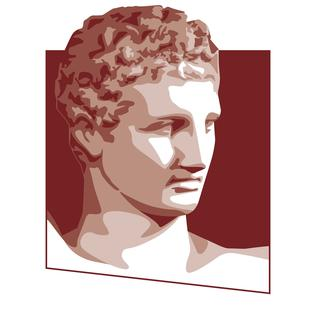
\includegraphics[width=0.4\textwidth]{titlepage_image}
	% Fill empty space
	\vfill

        \Large
        Management Science and Technology\\
        Athens University of Economics and Business\\
        Greece\\
	% Date goes here
        DD/MM/YYYY
	% You can adjust the space here
	\vspace{2.5cm}
 
    \end{center}
\end{titlepage}
% Insert abstract
\begin{center}
    % Make all titles large
    \LARGE
    % Thesis title goes here
    \themebold{My thesis title} \\
    % You can adjust the space here
     \vspace{0.5cm}
    % If there is a thesis subtitle (e.g. case study name), it goes here
    My thesis subtitle \\
    % You can adjust the space here
    \vspace{0.4cm}
    % Full name goes here
    \themebold{Full Name} \\
    % You can adjust the space here
    \vspace{1.5cm}
    \themebold{Abstract} 
\\
% You can adjust the space here
\vspace{25mm}
\end{center}
% Center paragraph
\begin{center}
Your abstract is simply a short, stand-alone summary of the thesis that others can use as an overview. It is recommended that you first finish writing your thesis and then write this part. Keep in mind to inform the reader about the problem you recognised, the purpose of your thesis, the process you are following and your conclusions.
\end{center}
\vfill
% Insert table of contents
\tableofcontents

% ---- Insert chapter titles and text ----
\chapter{FIRST CHAPTER}
\section{LATEX}

\subsection{Basics}
\begin{itemize}
\item To run your code and produce the pdf file or update it run the following command: \\
\begin{lstlisting}[language=bash]
  $ pdflatex thesis
\end{lstlisting}
\item To create sections you add \verb|\section{Section's name}|.
\item To add subsections you add \verb|\subsection{Subsection's name}|.
\item For line break you use \verb|\\|.
\item To center text you can either use \verb|\centering| or wrap your text around \verb|\begin{center}| and \verb|\end{center}| (example in abstract).
\item To reference another part of the document, like a chapter, a figure, a table, you need to set a label for that part and then use \verb|\ref{part's label}|. It will look like this: \ref{citations}.
\end{itemize}

\subsection{Citations}
\label{citations}
In order to create citations you first need to include your sources in bibliography.bib file. The first attribute of each source is set by you and is basically an identification for the corresponding source. To cite you use that attribute. 
\begin{itemize}
\item In case you want to mention the name of the author (for example in the beginning of a paragraph), you can use \verb|\textcite{textciteExample}| and it will look like this \textcite{bookExample}. 
\item In case you want to make the complete citation you can use \verb|\autocite{autociteExample}| and it would look like this \autocite{articleExample}.
\item To refer to specific pages you can add the pages inside brackets. \verb|\autocite[1]{example}| for single page or \verb|\autocite[1-2]{example}| for multiple pages. They should look like this, \autocite[1]{articleExample} and \autocite[1-2]{bookExample}.
\item Whenever you add a new source in your bibliography.bib file and add a citation, you need to run the following sequence on your cmd: \\
\begin{lstlisting}[language=bash]
  $ pdflatex thesis
  $ biber thesis
  $ pdflatex thesis
\end{lstlisting}
\item You can include multiple authors separating them by and. For example 'John Doe and Jane Doe'.
\end{itemize}

\subsection{Bulleted Lists}
You can create bulleted lists by including your text inside \verb|\begin{itemize}| and \verb|\end{itemize}|. Start each bulltet point with \verb|\item|. \\
% Create bulleted list
\begin{itemize}
% First item
\item Lorem ipsum dolor sit amet, consectetur adipiscing elit, sed do eiusmod tempor incididunt ut labore et dolore magna aliqua. Ut enim ad minim veniam, quis nostrud exercitation ullamco laboris nisi ut aliquip ex ea commodo consequat. Duis aute irure dolor in reprehenderit in voluptate velit esse cillum dolore eu fugiat nulla pariatur. Excepteur sint occaecat cupidatat non proident, sunt in culpa qui officia deserunt mollit anim id est laborum. \\
% Second item
\item Lorem ipsum dolor sit amet, consectetur adipiscing elit, sed do eiusmod tempor incididunt ut labore et dolore magna aliqua. Ut enim ad minim veniam, quis nostrud exercitation ullamco laboris nisi ut aliquip ex ea commodo consequat. Duis aute irure dolor in reprehenderit in voluptate velit esse cillum dolore eu fugiat nulla pariatur. Excepteur sint occaecat cupidatat non proident, sunt in culpa qui officia deserunt mollit anim id est laborum. \\
% Third item
\item Lorem ipsum dolor sit amet, consectetur adipiscing elit, sed do eiusmod tempor incididunt ut labore et dolore magna aliqua. Ut enim ad minim veniam, quis nostrud exercitation ullamco laboris nisi ut aliquip ex ea commodo consequat. Duis aute irure dolor in reprehenderit in voluptate velit esse cillum dolore eu fugiat nulla pariatur. Excepteur sint occaecat cupidatat non proident, sunt in culpa qui officia deserunt mollit anim id est laborum.
% Fourth item
\item Lorem ipsum dolor sit amet, consectetur adipiscing elit, sed do eiusmod tempor incididunt ut labore et dolore magna aliqua. Ut enim ad minim veniam, quis nostrud exercitation ullamco laboris nisi ut aliquip ex ea commodo consequat. Duis aute irure dolor in reprehenderit in voluptate velit esse cillum dolore eu fugiat nulla pariatur. Excepteur sint occaecat cupidatat non proident, sunt in culpa qui officia deserunt mollit anim id est laborum.
% End of bulleted list
\end{itemize}

\section{Figures}
% Example of how to reference a figure inside text
You can reference figures inside text using \verb|\ref| and the figure label inside curly brackets like this \verb|\ref{image_label}| and the result looks like this \ref{fig:image}. \\

A single figure look as follows:\\
% Example of how to insert a figure
\begin{figure}[ht]
% You can justify image width and height here, put the name of your image inside the curly brackets
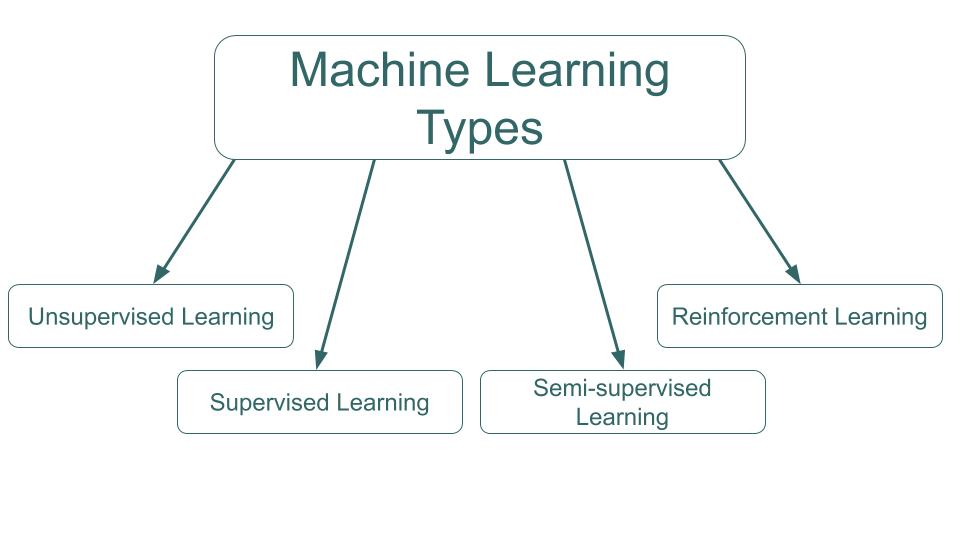
\includegraphics[width=\textwidth]{figure}
% Image caption
\caption{My caption.}
% Label is used to reference image inside text as shown above
\label{fig:image}
\end{figure}
\\
You also have the ability to add two images in the same figure. Depending on which label you are using, you can reference the whole figure \ref{fig:double_image}, or the images seperately \ref{fig:first_image}, \ref{fig:second_image}. The figure looks as follows:
% Example of how to insert a figure with two images
\begin{figure}[ht]
\centering
% Setting width to be half the total line width (because there are two images), you can customize it
\begin{subfigure}{.5\textwidth}
\centering
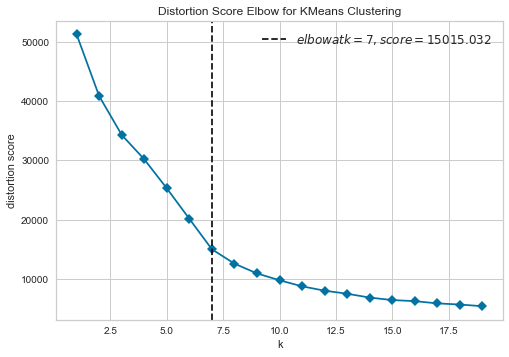
\includegraphics[width=\linewidth]{first_image}
\caption{First image caption.}
\label{fig:first_image}
\end{subfigure}%
% Setting width to be half the total line width (because there are two images), you can customize it
\begin{subfigure}{.5\textwidth}
\centering
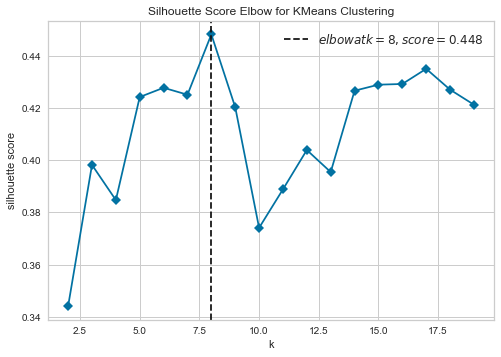
\includegraphics[width=\linewidth]{second_image}
\caption{Second image caption.}
\label{fig:second_image}
\end{subfigure}%
\caption{General caption for both figures.}
\label{fig:double_image}
\end{figure}
\\

\section{Mathematics and Algorithms}
In case you want to write mathematical equations, you can do this either inline, or using the equation display. \\
To enter math mode inline you need to include text between \verb|\(| and \verb|\)|, for example to print \(2^{3}\) you should write \verb|\(2^{3}\)|. \\
In case you would like to use equation display you need to wrap your equations around \verb|\begin{eqnarray*}| and \verb|end{eqnarray*}|. The equation would look like this:
\begin{eqnarray*}
d_{ij} = \sqrt{(c_{i}-x_{j})^2}
\end{eqnarray*}
\\
There is a large amount of math symbols that you can use to write your equations, too many to mention here, but if you google latex math symbols you should be able to find many cheat sheets to help you complete your equations. \\

To write pseudocode you can wrap your text around \verb|\begin{algorithm}| and \verb|\end{algorithm}|. To write the expected input you can write \verb|\KwInput{input}| and the expected output using \verb|\KwOutput{output}|. \\
An example is illustrated below:
% Example of how to write pseudocode
\begin{algorithm}
\SetAlgoLined
% Define your input here
\KwInput{\(D=\{x_{1},x_{2},...,x_{n}\} \)\newline
K initial centroids
}
% Define your output here
\KwOutput{K cluster sets}
% Create a while loop
\While{termination condition is not reached}
{
Assign each element to the cluster of the closest centroid.\\
Recompute the new centroids.
}
% The label can be used to reference the algorithm with \ref
\caption{Kmeans}\label{alg:kmeans}
\end{algorithm} 

\chapter{SECOND CHAPTER}
\section{First Section}
Lorem ipsum dolor sit amet, consectetur adipiscing elit, sed do eiusmod tempor incididunt ut labore et dolore magna aliqua. Ut enim ad minim veniam, quis nostrud exercitation ullamco laboris nisi ut aliquip ex ea commodo consequat. Duis aute irure dolor in reprehenderit in voluptate velit esse cillum dolore eu fugiat nulla pariatur. Excepteur sint occaecat cupidatat non proident, sunt in culpa qui officia deserunt mollit anim id est laborum. \\
Lorem ipsum dolor sit amet, consectetur adipiscing elit, sed do eiusmod tempor incididunt ut labore et dolore magna aliqua. Ut enim ad minim veniam, quis nostrud exercitation ullamco laboris nisi ut aliquip ex ea commodo consequat. Duis aute irure dolor in reprehenderit in voluptate velit esse cillum dolore eu fugiat nulla pariatur. Excepteur sint occaecat cupidatat non proident, sunt in culpa qui officia deserunt mollit anim id est laborum. \\
Lorem ipsum dolor sit amet, consectetur adipiscing elit, sed do eiusmod tempor incididunt ut labore et dolore magna aliqua. Ut enim ad minim veniam, quis nostrud exercitation ullamco laboris nisi ut aliquip ex ea commodo consequat. Duis aute irure dolor in reprehenderit in voluptate velit esse cillum dolore eu fugiat nulla pariatur. Excepteur sint occaecat cupidatat non proident, sunt in culpa qui officia deserunt mollit anim id est laborum. \\
\section{Second Section}
Lorem ipsum dolor sit amet, consectetur adipiscing elit, sed do eiusmod tempor incididunt ut labore et dolore magna aliqua. Ut enim ad minim veniam, quis nostrud exercitation ullamco laboris nisi ut aliquip ex ea commodo consequat. Duis aute irure dolor in reprehenderit in voluptate velit esse cillum dolore eu fugiat nulla pariatur. Excepteur sint occaecat cupidatat non proident, sunt in culpa qui officia deserunt mollit anim id est laborum.
\section{Third Section}
Lorem ipsum dolor sit amet, consectetur adipiscing elit, sed do eiusmod tempor incididunt ut labore et dolore magna aliqua. Ut enim ad minim veniam, quis nostrud exercitation ullamco laboris nisi ut aliquip ex ea commodo consequat. Duis aute irure dolor in reprehenderit in voluptate velit esse cillum dolore eu fugiat nulla pariatur. Excepteur sint occaecat cupidatat non proident, sunt in culpa qui officia deserunt mollit anim id est laborum.

\chapter{THIRD CHAPTER}
\section{First Section}
Lorem ipsum dolor sit amet, consectetur adipiscing elit, sed do eiusmod tempor incididunt ut labore et dolore magna aliqua. Ut enim ad minim veniam, quis nostrud exercitation ullamco laboris nisi ut aliquip ex ea commodo consequat. Duis aute irure dolor in reprehenderit in voluptate velit esse cillum dolore eu fugiat nulla pariatur. Excepteur sint occaecat cupidatat non proident, sunt in culpa qui officia deserunt mollit anim id est laborum. \\
Lorem ipsum dolor sit amet, consectetur adipiscing elit, sed do eiusmod tempor incididunt ut labore et dolore magna aliqua. Ut enim ad minim veniam, quis nostrud exercitation ullamco laboris nisi ut aliquip ex ea commodo consequat. Duis aute irure dolor in reprehenderit in voluptate velit esse cillum dolore eu fugiat nulla pariatur. Excepteur sint occaecat cupidatat non proident, sunt in culpa qui officia deserunt mollit anim id est laborum. \\
Lorem ipsum dolor sit amet, consectetur adipiscing elit, sed do eiusmod tempor incididunt ut labore et dolore magna aliqua. Ut enim ad minim veniam, quis nostrud exercitation ullamco laboris nisi ut aliquip ex ea commodo consequat. Duis aute irure dolor in reprehenderit in voluptate velit esse cillum dolore eu fugiat nulla pariatur. Excepteur sint occaecat cupidatat non proident, sunt in culpa qui officia deserunt mollit anim id est laborum. \\
\section{Second Section}
Lorem ipsum dolor sit amet, consectetur adipiscing elit, sed do eiusmod tempor incididunt ut labore et dolore magna aliqua. Ut enim ad minim veniam, quis nostrud exercitation ullamco laboris nisi ut aliquip ex ea commodo consequat. Duis aute irure dolor in reprehenderit in voluptate velit esse cillum dolore eu fugiat nulla pariatur. Excepteur sint occaecat cupidatat non proident, sunt in culpa qui officia deserunt mollit anim id est laborum.
\section{Third Section}
Lorem ipsum dolor sit amet, consectetur adipiscing elit, sed do eiusmod tempor incididunt ut labore et dolore magna aliqua. Ut enim ad minim veniam, quis nostrud exercitation ullamco laboris nisi ut aliquip ex ea commodo consequat. Duis aute irure dolor in reprehenderit in voluptate velit esse cillum dolore eu fugiat nulla pariatur. Excepteur sint occaecat cupidatat non proident, sunt in culpa qui officia deserunt mollit anim id est laborum.

\chapter{CONCLUSIONS}
\section{First Section}
Lorem ipsum dolor sit amet, consectetur adipiscing elit, sed do eiusmod tempor incididunt ut labore et dolore magna aliqua. Ut enim ad minim veniam, quis nostrud exercitation ullamco laboris nisi ut aliquip ex ea commodo consequat. Duis aute irure dolor in reprehenderit in voluptate velit esse cillum dolore eu fugiat nulla pariatur. Excepteur sint occaecat cupidatat non proident, sunt in culpa qui officia deserunt mollit anim id est laborum. 
\section{Second Section}
Lorem ipsum dolor sit amet, consectetur adipiscing elit, sed do eiusmod tempor incididunt ut labore et dolore magna aliqua. Ut enim ad minim veniam, quis nostrud exercitation ullamco laboris nisi ut aliquip ex ea commodo consequat. Duis aute irure dolor in reprehenderit in voluptate velit esse cillum dolore eu fugiat nulla pariatur. Excepteur sint occaecat cupidatat non proident, sunt in culpa qui officia deserunt mollit anim id est laborum. 
\section{Third Section}
Lorem ipsum dolor sit amet, consectetur adipiscing elit, sed do eiusmod tempor incididunt ut labore et dolore magna aliqua. Ut enim ad minim veniam, quis nostrud exercitation ullamco laboris nisi ut aliquip ex ea commodo consequat. Duis aute irure dolor in reprehenderit in voluptate velit esse cillum dolore eu fugiat nulla pariatur. Excepteur sint occaecat cupidatat non proident, sunt in culpa qui officia deserunt mollit anim id est laborum. 
% ------------------------------------------

% Prints bibliography page
\printbibliography
% Include bibliography to contents
\addcontentsline{toc}{section}{Bibliography}
\end{document}